\subsection{Préprocessamento}
	\label{subsec:preprocessamento}



	Os algoritmos \textit{TextTiling} e \textit{C99} foram propostos para o inglês e sem domínio determinado, ou seja, a proposta inicial é trabalhar em qualquer texto nessa língua.
	A proposta desse trabalho é adaptá-los ao contexto das atas de reunião em português do Brasil. As subseções seguintes tratam das adaptações para esse nicho mais específico. A seção~\ref{sec:avaliacao} mostra a análise dos algoritmos adaptados.


  \begin{figure}[!h]

	\centering
	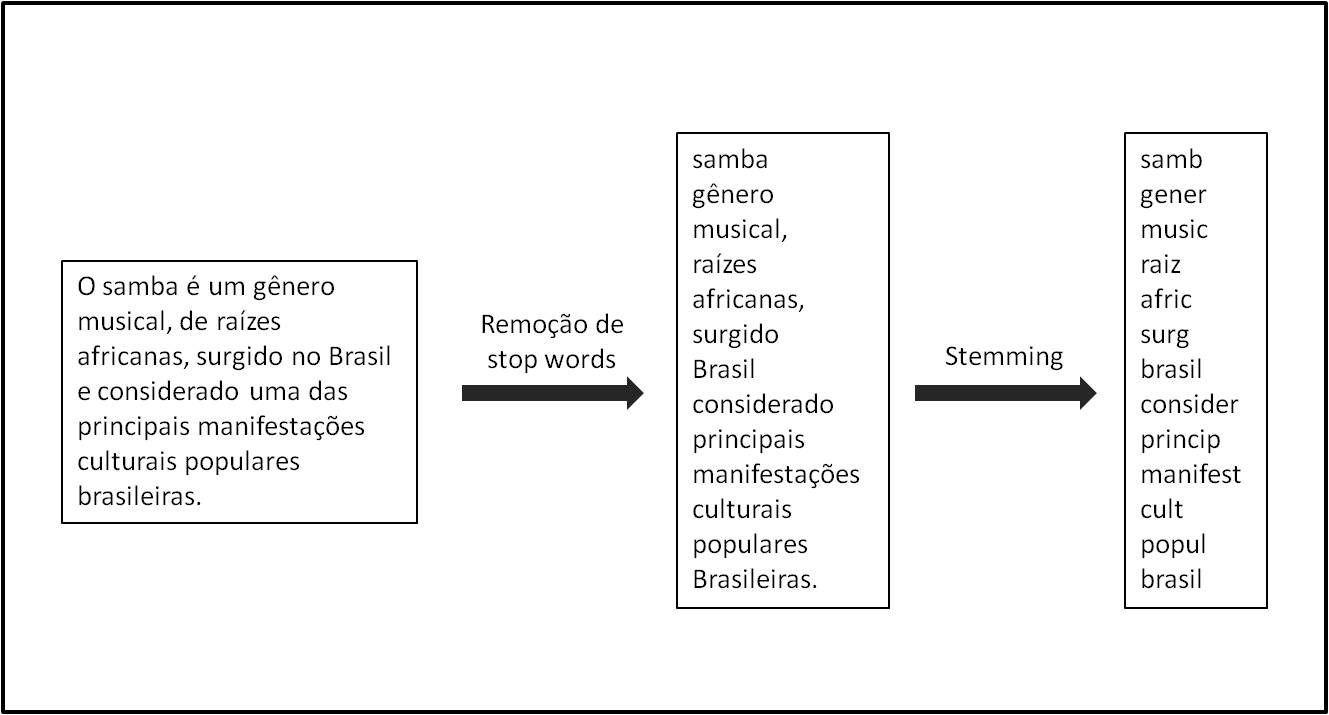
\includegraphics[width=0.45\textwidth]{exemplo-preprocessamento.jpg}
	\caption{Exemplo de preprocessamento}
	\label{fig:exemplomatrixrank}


	A etapa de pre-processamento, em um documento contendo texto puro, acontece em dois passos principais. Primeiro elimina-se as palavras consideradas menos informativas, as quais são chamadas de \textit{stop words}, para isso, utiliza-se uma lista contendo 438 palavras. Em seguida, remove-se os sufixos das palavras restantes, mantendo apenas o radical da


	\subsubsection{Remoção de ruídos}
		passos menores
		1 - heurística simples para remover cabeçalho e rodapé.
		2 - remoção de numerais
		3 - remoção de acentos, transformações de caixa, remoção de pontuação.
		
	% Esses passos são realizados internamente em cada algorímo, para que a saida seja legível ao usuário final.

  \end{figure}




	

\subsection{Identificação de sentenças}
	\label{subsec:indentificacaosentencas}


